\subsection{Cellular Networks}


\begin{figure*}[!ht]
    \centering
    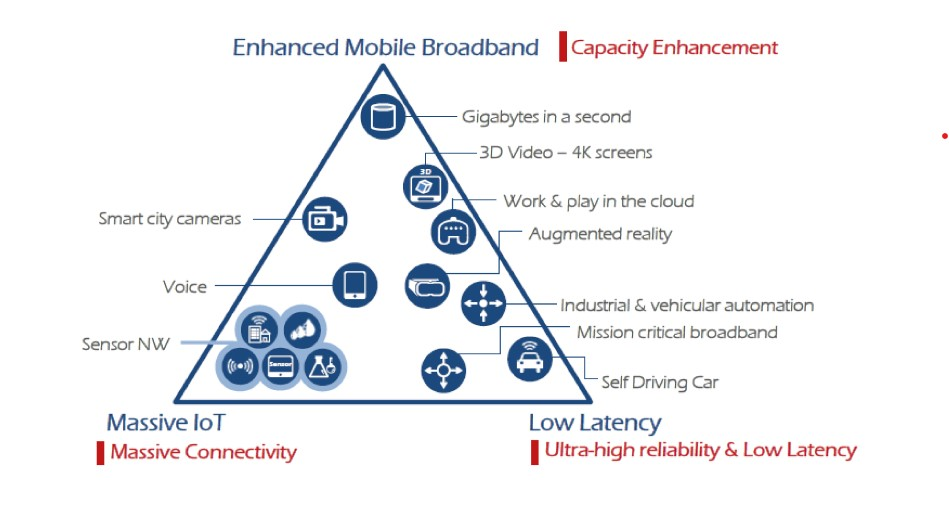
\includegraphics[width=.8\linewidth]{imgs/chapter_1/5g_app.jpg}
    \caption{ITU-T 5G requirements \protect{\cite{IMT_itut_2020}}}
    \label{fig:chap_1:5g_requirement}
\end{figure*}


Since the 1980s and the announcement of the 1st generation (1G) with a data rate of up to 2.4 kbps, each decade has seen the introduction of a new mobile cellular generation. The second generation (2G), launched in the 1990s, brought significant advancements over 1G, including services like \ac{SMS} text messaging. 2G supported communication with data rates of up to 144 kbps. 

The 3rd generation (3G), introduced in the 2000s, offered data rates ranging from 384 kbps to 42 Mbps (with its latest enhancements). 3G enabled new capabilities, such as convenient web browsing, and became the first cellular network widely adopted for diverse applications, including medical devices and fire alarms.

The 4th generation (4G), launched in the 2010s, was expanded by the \ac{ITU} to include the latest evolutions of 3G, such as \ac{LTE}, \ac{WiMAX}, and \ac{HSPA+}. It achieved speeds of up to 150 Mbps and featured reduced latency, improving the user experience for applications like video streaming, video conferencing, and gaming services.

The 5th generation (5G) began deployment in 2019, following its definition by \ac{3GPP} Release 15, which introduced \ac{5G NR} % add reference. 
Compared to LTE, 5G is expected to deliver up to 20 times the theoretical bandwidth of LTE (1 Gbps) and ultra-low latency down to 1 ms \cite{IMT_itut_2020}. 

5G is designed to address three key application scenarios, as illustrated in \ref{fig:chap_1:5g_requirement}:
\begin{itemize}
    \item \ac{eMBB}, providing faster connections with higher bandwidth (up to 20 Gbps) and moderate latency, suitable for applications like AR/VR, cloud gaming, and 360-degree video streaming.
    \item \ac{URLLC}, supporting ultra-low latency (down to 1 ms) and high reliability (99.999\%) for mission-critical applications, such as Industry 4.0 processes and remote healthcare.
    \item \ac{mMTC}, enabling connectivity for a large number of \ac{IoT} devices (up to $10^6$ per square kilometer), albeit with trade-offs in throughput and latency.
\end{itemize}


\subsubsection{Architecture of 4G/5G networks}



\begin{figure*}[!ht]
    \centering
    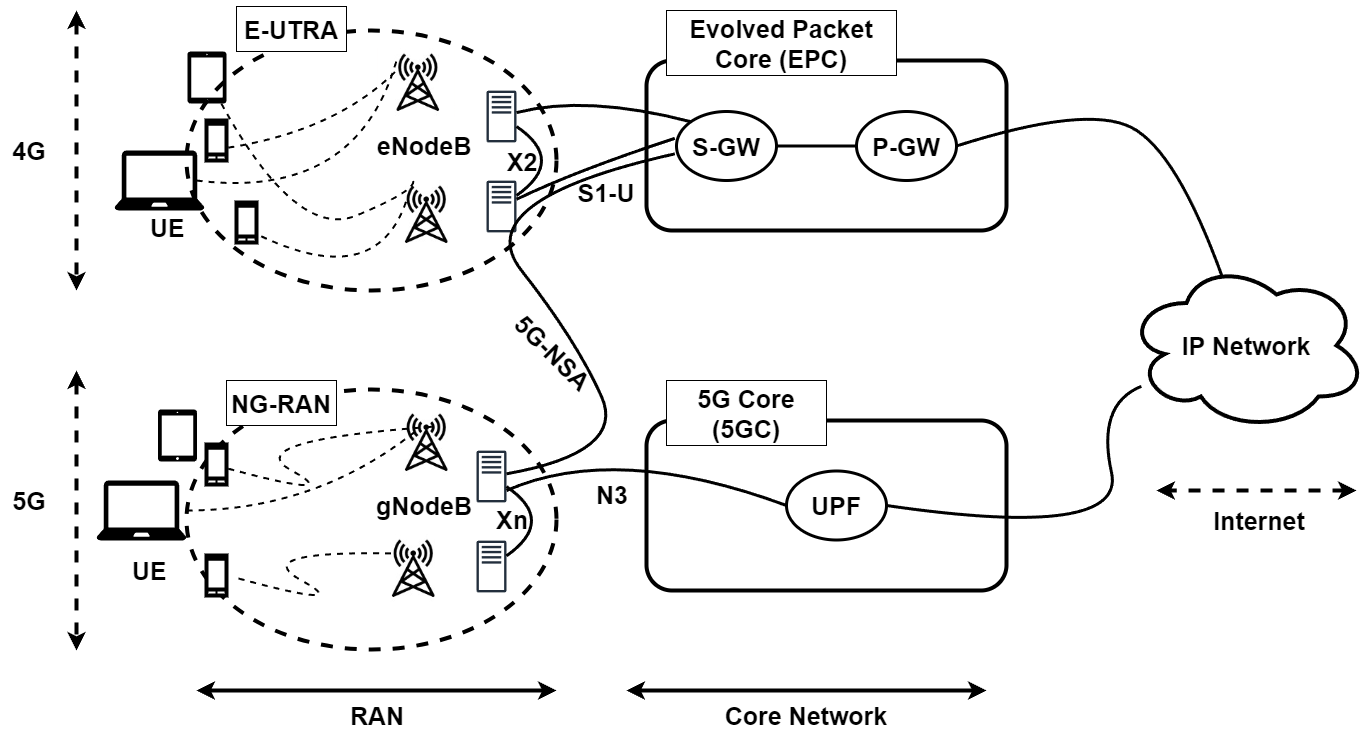
\includegraphics[width=.8\linewidth]{imgs/chapter_1/cellular_network.png}
    \caption{Cellular networks architecture (focus on user-plane)}
    \label{fig:chap_1:cellular_network}
\end{figure*}

The architecture of a cellular network, depicted in Fig. \ref{fig:chap_1:cellular_network}, consists of three main parts: the \ac{UE}, \ac{RAN}, and the core network. The core network connects the RAN to external networks (e.g., \ac{IP} networks), while the RAN provides connectivity between UEs and the mobile core network. In 4G (resp. 5G), the RAN is referred to as \ac{E-UTRA} (resp. \ac{NG-RAN}), and the mobile core network is known as \ac{EPC} (resp. \ac{5GC}).

The primary component of the RAN is the \ac{BS}, referred to as \ac{eNB} in 4G and \ac{gNB} in 5G. UEs connect to the BS through the radio air interface, and the BSs are linked to the core network. In 4G, BSs are interconnected via the X2 interface (resp. Xn interface in 5G) to facilitate handovers between neighboring cells. They are connected to the core network via the S1 interface (resp. N3 interface in 5G). 

The 4G \ac{EPC} comprises several key components. The \ac{MME} handles user authentication, mobility management, and signaling. The \ac{S-GW} manages the user data plane, while the \ac{P-GW} serves as a gateway connecting the network to external IP networks. 

In contrast, the 5GC is designed to be more flexible and cloud-aligned using a \ac{SBA}, where network functions are decoupled and deployed as microservices using \ac{NFV}. Key components of the 5GC include the Access and Mobility Management Function (AMF), which replaces the MME in 4G and handles connectivity and mobility management; the User Plane Function (UPF), which assumes the data routing roles of the SGW and PGW; and the Session Management Function (SMF), which manages session establishment and \ac{QoS}. 

The 5G architecture introduces advanced concepts such as network slicing, \ac{MEC}, and the use of a wider range of frequency bands (e.g., mmWave) to achieve higher throughputs and lower latency, supporting next-generation applications like low-latency services. 

Early 5G deployments used the \ac{NSA} architecture, which leverages \ac{5G NR} in the RAN to enhance data speeds while relying on the 4G EPC for control plane functions. This approach enabled faster initial 5G rollouts by requiring fewer infrastructure changes. However, \ac{NSA} cannot deliver the full potential of 5G, such as ultra-low latency and network slicing. Full \ac{SA} deployments, which use 5G NR along with the cloud-native 5G core, are expected to realize the complete range of capabilities promised by 5G networks.



\subsection{Wi-Fi networks}

Wi-Fi is a trademark of the Wi-Fi Alliance, commonly used to refer to wireless \ac{LAN}s based on IEEE 802.11 standards. Wi-Fi is used to connect devices such as laptops, smartphones, \ac{IoT} devices, and gaming consoles to the Internet via a wireless router. It enables short-range wireless communication in environments such as campuses, homes, and restaurants. Any device capable of connecting to a wireless network is referred to as a station and is equipped with a wireless network interface controller. Stations are categorized into two types: \ac{AP}s and clients.



\subsubsection{Architecture of Wi-Fi networks}

Wi-Fi networks are primarily deployed in infrastructure mode, where all communications pass through an AP. In this mode, a Wi-Fi network architecture comprises one or more APs, one or more client devices connected to the AP, and a distribution system (typically a wired Ethernet connection) that links the AP to the Internet. The AP broadcasts to the clients a \ac{SSID} to identify the network, using beacon packets. To access the Internet, a client sends an association request to the AP, which authenticates the client using security protocols such as \ac{WPA} (e.g., WPA2/WPA3). Once authenticated, the client is assigned an IP address by the \ac{DHCP} server on the AP, enabling Internet connectivity.

% Figure architecture Wi-Fi


\subsubsection{Evolution of WiFi standards with performance characteristics}

The first Wi-Fi standard, IEEE 802.11, was released in 1997. Operating at 2.4 GHz, it offered data rates of up to 2 Mbps. However, it faced limited adoption due to interoperability issues, insufficient throughput, and weak security. In 1999, IEEE 802.11b (Wi-Fi 1) improved upon this by achieving theoretical data rates of up to 11 Mbps at 2.4 GHz and a range of up to 300 meters in clear environments. Wi-Fi 1 gained popularity for basic Internet browsing and email but suffered from interference issues due to sharing the 2.4 GHz band with other wireless technologies like Bluetooth and microwave ovens.

IEEE 802.11a (Wi-Fi 2) was introduced alongside Wi-Fi 1, operating on the less-crowded 5 GHz band with data rates of up to 54 Mbps. However, its higher frequency required more expensive antennas to maintain range, and it was not interoperable with Wi-Fi 1. 

In 2003, IEEE 802.11g (Wi-Fi 3) combined the strengths of 802.11b and 802.11a by operating on the 2.4 GHz band while offering data rates of up to 54 Mbps. It was backward compatible with 802.11b, making it a popular choice for commercial use.

Released in 2009, IEEE 802.11n (Wi-Fi 4) brought significant improvements in speed and reliability. It introduced \ac{MIMO} technology, allowing multiple antennas to transmit and receive data simultaneously, achieving data rates of up to 600 Mbps. It also supported dual-band support (2.4 and 5 GHz), offering better range and reduced interference.

Built on the advancements of 802.11n, IEEE 802.11ac (Wi-Fi 5), launched in 2013, further enhanced Wi-Fi performance by operating exclusively on the 5 GHz band, offering gigabit speeds of up to 3.5 Gbps. Features such as advanced MIMO configurations, beamforming, and wider channel bandwidths made it ideal for applications like \ac{HD} and 4K video streaming, gaming, and video conferencing. It remained backward compatible with previous standards.

IEEE 802.11ax (Wi-Fi 6 and later Wi-Fi 6E) improved performance, scalability, and energy efficiency with \ac{OFDMA} technology. Wi-Fi 6 operates on the 2.4 GHz and 5 GHz bands, while Wi-Fi 6E adds the 6 GHz band, providing additional spectrum and reducing congestion. With speeds of up to 9.6 Gbps, this standard is ideal for environments with many connected devices, such as smart homes and IoT ecosystems.

The upcoming IEEE 802.11be (Wi-Fi 7) standard aims to further enhance performance, delivering data rates of up to 46 Gbps and ultra-low latency. It is designed to support advanced applications like AR/VR, 8K streaming, and immersive experiences.

The evolution of Wi-Fi standards is summarized in Tab. \ref{tab:wifi_standard}.

\begin{table*}[!h]
\setlength\tabcolsep{1pt} 
    
\begin{tabular*}{\linewidth}{@{\extracolsep{\fill}} lccccc}
    \toprule
       & \bf IEEE 802.11 & \bf Release & \bf Frequency & \bf Channel & \bf Max \\
       & \bf protocol & \bf Date & \bf Band (GHz) & \bf Bandwidth (MHz) & \bf Throughput \\
    \addlinespace
    \cmidrule{1-6}
            & 802.11 & 1997 & 2.4 & 22 & 2 Mbps \\
    Wi-Fi 1 & 802.11b & 1999 & 2.4 & 22 & 11 Mbps \\
    Wi-Fi 2 & 802.11a & 1999 & 5 & 20 & 54 Mbps \\
    Wi-Fi 3 & 802.11g & 2003 & 2.4 & 20 & 54 Mbps \\
    Wi-Fi 4 & 802.11n & 2009 & 2.4 & 20/40 & 600 Mbps \\
    Wi-Fi 5 & 802.11ac & 2013 & 5 & 20/40/80/160 & 3.5 Gbps \\
    Wi-Fi 6 & 802.11ax & 2019 & 2.4/5 & 20/40/80/160 & 9.6 Gbps\\
    Wi-Fi 6E & 802.11ax & 2020 & 2.5/5/6 & 20/40/80/160 & 9.6 Gbps \\
    Wi-Fi 7 & 802.11be & 2024 (expected) & 2.5/5/6 & 20/40/80/160/320 & 46.1 Gbps \\
    \bottomrule

\end{tabular*}
\caption{Evolution of Wi-Fi standards}
\label{tab:wifi_standard}
\end{table*}
% https://www.wevolver.com/article/the-evolution-of-wi-fi-networks-from-ieee-80211-to-wi-fi-6e


\subsection{LL applications performance under time-varying capacity network}
Low-latency applications such as CG and Cloud VR require high-performance networks to ensure acceptable \ac{QoS}/\ac{QoE}. However, their performance is significantly affected by time-varying network capacity. This section synthesizes insights from the literature on how CG and Cloud VR perform under such network conditions.

\subsubsection{Performance on cellular networks}
Kamarainen et al. \cite{Kmrinen2017AMS} found that LTE networks deliver stable network delays under strong signal conditions (RSRP between -50 and -70 dBm). However, noticeable delay fluctuations occur with weaker signals (-100 dBm or more), and latency can increase 2-4 times under poor conditions.
Domenico et al. \cite{Domenico2021ANA} examined cloud gaming performance on 3G and 4G networks using \ac{STD} as a benchmark. They observed that STD struggles to stream on 3G, even under optimal conditions. In contrast, 4G networks can support resolutions up to 4K with excellent signal quality, although poor 4G conditions lead to abrupt streaming interruptions.
Tan et al. \cite{tan2018supporting} highlighted LTE’s signaling inefficiencies, such as inter-protocol incoordinations and single-protocol overhead, which contribute to network latency often exceeding the 25 ms threshold required for acceptable VR performance.
Bhuyan et al. \cite{bhuyan2022end} demonstrated that 5G networks can handle 4K CG streams with high bitrates (up to 50 Mbps). However, frame drops occur due to larger game frame sizes and buffering-induced packet loss. These frame drops are significantly reduced when the bitrate is lowered to 30 Mbps. The study also revealed that 5G is 46\% more energy-intensive than Wi-Fi, mainly due to its use of higher frequencies and the power demands of mmWave antennas.
Penaherrera et al. \cite{penaherrera2024cloud} validated that standalone 5G (5G SA) networks effectively support Cloud VR applications. However, combining 5G SA with WiFi 6 increases latency due to Wi-Fi's higher uplink latency in WiFi. In mobility scenarios, 5G outperforms WiFi by offering higher throughput and more stable latencies.


\subsubsection{Performance on WiFi networks}
Maiorano et al. \cite{maiorano2022local} demonstrated that the performance of Cloud VR applications, such as NVIDIA’s CloudXR, deteriorates as the distance between the headset and router increases. Low bandwidth reduces frame rates while signal attenuation increases delay.
Zhang et al. \cite{zhang2018wifi} revealed that Wi-Fi 5 struggles with Cloud VR due to high \ac{RTT} of up to 228 ms and jitter levels that exceed the recommended thresholds for real-time applications.
Jansen et al. \cite{jansen2023can} showed that signal attenuation on Wi-Fi networks causes bandwidth fluctuations, destabilizing throughput and affecting Cloud VR performance. The 5 GHz band offers higher bandwidth than the 2.4 GHz band but is more susceptible to signal attenuation.
Penaherrera et al. \cite{penaherrera2024cloud} demonstrated that Wi-Fi 6 provides superior latency performance for Cloud VR compared to 5G in stationary scenarios. However, its uplink performance remains a limiting factor.
Burbano et al. \cite{burbano2024impact} emphasized that even Wi-Fi 6 struggles to maintain stable Cloud VR sessions under high traffic congestion, particularly on the 2.4 GHz band.



\subsubsection{Key Observations Across Networks}

Studies such as \cite{Domenico2021ANA, bhuyan2022end} emphasize the importance of adequate bandwidth in ensuring the performance of low-latency applications. While 5G offers superior capacity, Wi-Fi remains limited by its inherent constraints, especially in older protocols. Cellular networks, particularly 5G, excel in providing low-latency connections. However, inefficiencies in LTE protocols and signal attenuation in Wi-Fi can significantly degrade performance. Additionally, \cite{bhuyan2022end} highlights that Wi-Fi is more energy-efficient than 5G for CG and Cloud VR, making it more suitable for stationary use cases. Finally, the performance of both 4G and Wi-Fi is heavily dependent on signal quality, with poor conditions exacerbating latency, jitter, and packet loss.



%\takeaway{Cellular networks offer varying levels of bandwidth and latency, with 5G enabling ultra-low latency for mission-critical applications. Wi-Fi protocols have evolved to support higher data rates. However, user experience of LL applications under these networks are often challenging as  time-varying capacity networks may present bandwidth unavailability and latency instability due to multiple causes.} % change suboptimal


% \takeaway{Cellular networks have evolved from 1G to 5G, with 5G offering ultra-low latency, enhanced bandwidth, and novel concepts like network slicing and edge computing. Similarly, Wi-Fi standards have progressed from IEEE 802.11 to Wi-Fi 7, delivering higher throughput and reduced latency. Despite these advancements, both network types face multiple challenges resulting in bandwidth unavailability and latency instability, which impact performance of \ac{LL} applications.}



% \usage{This thesis focuses on evaluating \ac{LL} applications under challenging network environments, specifically 4G and Wi-Fi. The experimental testbeds for data collection (Chapter \ref{chap:measurements}) were designed to reproduce realistic scenarios within these networks, thus capturing the performance impacts and challenges faced by LL applications in such environments.}
 








    
    % Jansen et al. Can My WiFi Handle the Metaverse? A Performance Evaluation Of Meta’s Flagship Virtual Reality Hardware
    
    % Casasnovas et al. Experimental evaluation of interactive Edge/Cloud Virtual Reality gaming over Wi-Fi using unity render streaming

    % Penaherrera et al. \cite{penaherrera2022kqi} KQI Assessment of VR Services: A Case Study on 360-Video Over 4G and 5G





    % Michaelides et al. Is Wi-Fi 6 Ready for Virtual Reality Mayhem? A Case Study Using One AP and Three HMDs

